\documentclass[12pt]{article}
\title{ECE 3 Lab 1 prelab}

\author{Lawrence Liu}
\usepackage{graphicx}
\usepackage{amsmath}
\setlength{\parindent}{0pt}
\usepackage[section]{placeins}
\begin{document}
\maketitle
\section*{Problem 1}
\subsection*{(a)}
$47k\Omega$ with variance of $5\%$
\subsection*{(b)}
$100k\Omega$ with variance of $10\%$
\section*{Problem 2}
$0\Omega$ because the resistor is parallel with a short circuit, to properly measure the resistance you should plug in the resistor with B one row back.
\section*{Problem 3}
\subsection*{Ideal Voltage Source}
\begin{figure}[h]
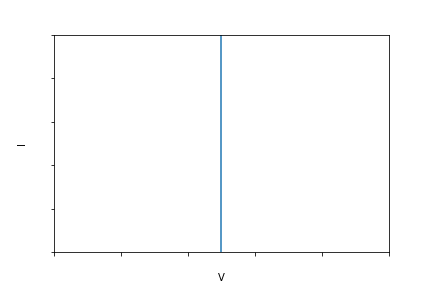
\includegraphics[scale=0.5]{fig1}
\centering
\end{figure}
\FloatBarrier
\subsection*{Non Ideal Voltage Source}
\begin{figure}[h]
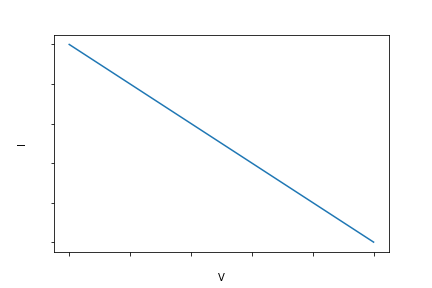
\includegraphics[scale=0.5]{fig3}
\centering
\end{figure}
\FloatBarrier
\subsection*{Ideal Current Source}
\begin{figure}[h]
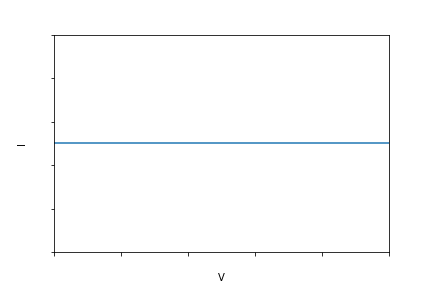
\includegraphics[scale=0.5]{fig2}
\centering
\end{figure}
\FloatBarrier
\subsection*{Non Ideal Current Source}
\begin{figure}[h]
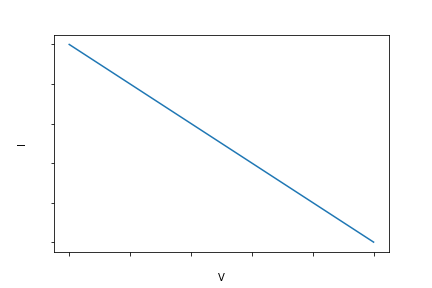
\includegraphics[scale=0.5]{fig4}
\centering
\end{figure}
\FloatBarrier
\section*{Problem 4}
\subsection*{Voltage Divider}
From KVL we have
$$V_0=I(R_1+R_2)$$
$$I=\frac{V_0}{R_1+R_2}$$
therefore we have that the voltage drop across $R_1$ is
$$\frac{V_0 R_1}{R_1+R_2}$$
\subsection*{Voltage Divider}
We have
$$V_0=I_T\frac{R_1R_2}{R_1+R_2}$$
therefore we have that the current across $R_1$ is
$$V_0=I_1 R_1$$
$$I_T\frac{R_1R_2}{R_1+R_2}=I_1R_1$$
$$I_T\frac{R_2}{R_1+R_2}=I_1$$

\end{document}